\section{Durchführung}
\label{sec:Durchführung}
Wesentliche Bestandteile des Aufbaus sind eine Kupfer-Röntgenröhre, ein LiF-Kristall bzw. ein Plexiglas-Streuer und ein Geiger-Müller-Zählrohr.
In dem Gerät, welches in Abbildung \ref{fig:rön} zu sehen ist, ist die Elektronik integriert. Das Emissionsspektrum und die Transmission $T(\lambda)$ des Aluminium-Absorbers wird mit dem Rechner vermessen.
\begin{figure}
    \centering
    \caption{Röntgenröhre.\cite{V603}}
    \label{fig:rön}
    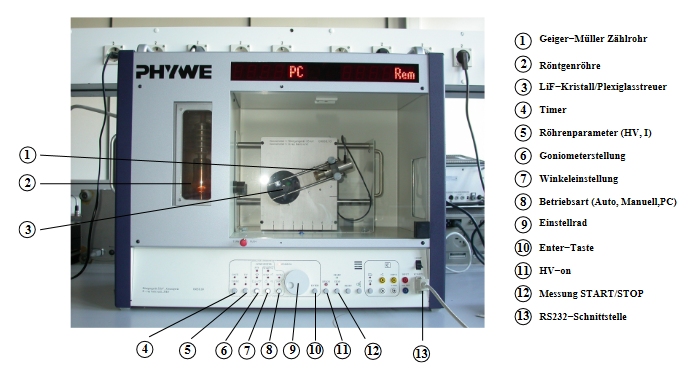
\includegraphics[width = 0.6 \textwidth]{pics/röntgenröhre.png}
\end{figure}
Für die Bestimmung der Compton-Wellenlänge wird eine manuelle Bedienung genutzt. Es wird eine Beschleunigungsspannung von $\SI{35}{\kilo \volt}$ mit einem Emissionsstrom von $\SI{1}{\milli \ampere}$ gewählt.
Der LiF-Kristall wird in die Halterung gesteckt. Eine $\SI{2}{\milli \metre}$ wird verwendet um das Emissionsspektrum aufzunehmen. In Schritten von $\symup{\Delta}\alpha=\ang{0.1;;}$ und einer Integrationszeit pro Winkel von $t=\SI{10}{\second}$
wird das Emissionsspektrum im Bereich von $\ang{8;;} \leq \alpha \leq \ang{25;;}$ gemessen. 
\\
Die Bestimmung der Transmission als Funktion der Wellenlänge wird in Schritten von $\symup{\Delta}\alpha=\ang{0.1;;}$ im Bereich $\ang{7;;} \leq \alpha \leq \ang{10;;}$ durchgeführt.
Dabei wird einmal ohne Aluminium-Absorber $N_\text{Al}(\theta)$ und einmal mit Aluminium-Absorber $N_0(\theta)$ die Zählrate der Röntgenstrahlung gemessen. Die Integrationszeit pro Winkel beträgt
$t=\SI{200}{\second}$. Die gemessenen Zählraten werden mit der Totzeitkorrektur des Geiger-Müller Zählrohrs
\begin{equation}
    I=\frac{N}{1-\tau N}
    \label{eqn:tot}
\end{equation}
korrigiert, dabei beträgt die Totzeit des Geiger-Müller Zählrohrs $\tau=\SI{90}{\micro \second}$.
In dem nächsten Versuchsteil wird die $\SI{2}{\milli \metre}$-Blende durch eine $\SI{5}{\milli \metre}$-Blende ersetzt. Des weiteren wird der LiF-Kristall
durch einen Plexiglas-Streuer ersetzt. Es werden Messdaten für die korrigierten Zählraten ohne Aluminium-Absorber $I_0$, mit Aluminium-Absorber zwischen Röntgenröhre und Streuer $I_1$ und mit Aluminium-Absorber zwischen Streuer und Geiger-Müller Zählrohr $I_2$ entnommen.
Dabei wird der Winkel des Kristalls auf $\ang{45;;}$ und der Winkel des Geiger-Müller Zählrohrs auf $\ang{90};;}$ eingestellt. Die Integrationszeit beträgt $t=\SI{300}{\second}$.


